\chapter{Probabilistic TFA of \textit{C. elegans}}

% **************************** Define Graphics Path **************************
\ifpdf
    \graphicspath{{Chapter2/Figs/Raster/}{Chapter2/Figs/PDF/}{Chapter2/Figs/}}
\else
    \graphicspath{{Chapter2/Figs/Vector/}{Chapter2/Figs/}}
\fi

The data – information – knowledge – wisdom (DIKW) hierarchy is one of the 
fundamental and widely recognized hierarchy in the information and knowledge literature.
This hierarchy contextualize data, information, knowledge, and wisdom, with respect to one 
another to identify and describe the processes involved in the transformation of lower level entity
of the hierarchy to a higher level one(\cite{Rowley:2007}). The increasing availability
of very high dimentional data with diverse characteristics and growing complexity playing
the vital role behind the recent advancement of machine learning techniques. 

Data from real world likely to suffer from quality issue for various reasons. 



\section{Latent Variable Model}
Latent variable models (LVMs) \cite{Bishop:1999} explain complex relations between multiple variables 
by simple relations between the variables and an underlying unobservable, i.e. latent structure.
Latent variable are typically included in statistical model for different statistical concepts, 
including representation the unobservable factors/covariates, missing data, random effects, finite 
mixtures, variations in hierarchical data, and clusters and many more.

A set of latent (or hidden, or directly not observable) variables $\textbf{X}$ that can be related 
to the observed variables $\textbf{Y}$ defines by a joint distribution over both. The latent space is 
controlled by a prior distribution $p\left(\textbf{X}\right)$ over the distribution of $\textbf{Y}$
under the assumption of a probabilistic mapping of the form:
\begin{equation} \label{eq:linear_model}
y_{i,j} = f_j\left(\textbf{x}_{i}\right) + \epsilon_{i},
\end{equation}
where $\textbf{x}_i \in \mathbb{R}^q$ is the latent point associated with the $i^th$ observation
$\textbf{y}_i \in \mathbb{R}^p$, $j$ is the index of the features of $\textbf{Y}$. Inaccuracy of
the model  and the noise of the data is modelled by the additional noise parameter $\epsilon_{i}$.
Typically it is assumed that the noise has a Gaussian distribution 
$\epsilon \sim \mathcal{N} \left(0,\beta^{-1}\right)$, where the term $\beta$ is the precision.

We can map $f$ of Equation \ref{eq:linear_model} as linear and equal to a matrix 
$\textbf{W}\in\mathbb{R}^{p\times q}$. Then we can rewrite the Equation \ref{eq:linear_model} as:
\begin{equation} \label{eq:linear_model_matrix}
y_{i,j} = w_j\left(\textbf{x}_{i}\right) + \epsilon_{i},
\end{equation}
where $w_j$ are the rows of $\textbf{W}$. This model is known as probabilistic version of principal 
component analysis (PPCA) \cite{Roweis:1998, Tipping:1999}. 

Given the prior distribution over the latent variables has a Gaussian distribution, then the 
precision $\beta$ can be infinity and PCA is recovered in the limit. The condiditioanl probablity
of the data given the latent space is:
\begin{equation} \label{eq:cond_prob_latent_space}
p\left(\textbf{y}_i|\textbf{x}_i,\textbf{W},\beta \right) = \mathcal{N} \left(\textbf{y}_i|\textbf{W}\textbf{x}_i,\beta^{-1}\textbf{I}\right).
\end{equation}
If we consider data points are independent, then the marginal likelihood of the data is obtained by:
\begin{equation} \label{eq:marginal_likelihood_latent_space}
p\left(\textbf{Y}|\textbf{W},\beta \right) = 
\int \prod^{N}_{i=1} p\left(\textbf{y}_i|\textbf{x}_i,\textbf{W},\beta\right)p\left(\textbf{x}_i\right)d\textbf{x}.
\end{equation}
Even for finite precision $\beta$ the maximum likelihood solution for $\textbf{W}$ spans the 
principal sub-space of the data \cite{Tipping:1999}. This approach is can be applicable for both 
linear (i.e.\ \cite{Sanguinetti:2006}) and non-linear (i.e.\ \cite{Lawrence:2005}) models.  

\begin{figure}
	\centering
		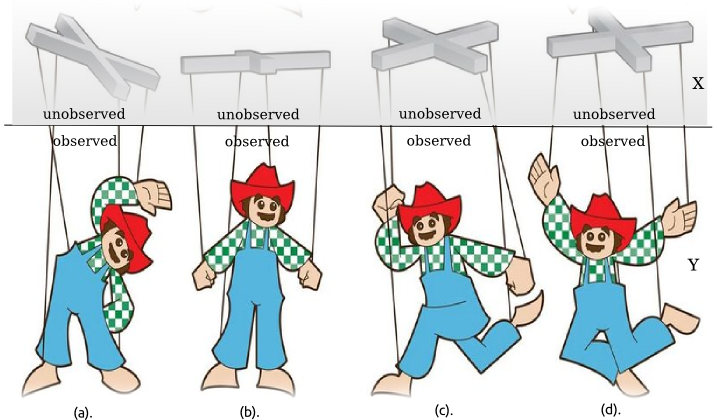
\includegraphics[width=0.7\textwidth,keepaspectratio]{LVM_Cartoon.png}
		\rule{35em}{0.5pt}
	\caption[Marionette Analogy of Latent Variable Model]
		{Marionette Analogy of Latent Variable Model}
	\label{fig:LVM Cartton}
\end{figure}


\section{Modelling of TFAs}
% %TODO
% 
% http://tex.stackexchange.com/questions/132526/overbrace-with-square-bracket
% \[
%  \overbrace{a+b+c}^{d} \quad \aoverbrace[L1R]{a+b+c}^{d} \quad
%  \underbrace{a+b+c}_{d} \quad \aunderbrace[l1r]{a+b+c}_{d}
% \]
%
% \section{Different models of TFAs}
In recent years most methods aim to infer a matrix of transcription factor activities (TFAs).
These TFAs are sum up in a single number at a certain experimental point to find 
the concentration of the transcription factor and its binding affinity to its target genes. 
Many of the researcher used different ways or algorithm to find out these TFAs. 
For example, \cite{Liao:2003} developed a data decomposition technique with dimension reduction and 
introduced ‘network component analysis’. This method takes account of the connectivity information 
by imposing algebraic constraints on the factors. They argued that classical statistical methods
such as principal component analysis and independent component analysis dose not consider the underlying 
network structure while computing low dimensional or hidden representation of a high-dimensional data sets 
like DNA microarray. 

\cite{Alter:2004} used a dimension reduction technique (SVD) to figure out TFAs and also the 
correlation between DNA replication initiation and RNA transcription during the yeast cell cycle. 
Using multivariate regression and backward variable selection 
to identify active transcription factors \cite{Gao:2004} targeted the same; 
\cite{Boulesteix:2005} used partial least squares (PLS) regression to infer the true TFAs 
from a combination of tRNA expression and DNA protein binding measurement. 
A major drawback of the above mentioned methods is that transcription factor activities do not 
hold any information regarding the strength of the regulators interactivity between the 
transcription factor and its different target genes. But it is expected that 
depending on the experimental conditions transcription factor activities can vary from gene to gene. 
Even it is also expected that different transcription factors may bind the same gene. 
In most of the cases, realistic information about the intervals may not be true as they were 
not based on fully probabilistic model. Moreover, false positives are always a problem for 
connectivity data, typically a large portion of Chip data suffers form it 
(\cite{Boulesteix:2005}). 
Furthermore, due to the various cellular process or changes in environmental conditions 
the structure of the regulatory network of the cell can change considerably.
Using regression-based methods it is difficult to track these changes. 
\cite{Nachman:2004} build a probabilistic model, using the basic framework of 
dynamic Bayesian networks using discrete random variables for protein concentrations 
and binding affinities. Though the model was more realistic but the computational complexity for 
genome-wide analysis can be expensive.

\subsection{Connectivity Information}
\cite{Xie:2005} used motif conservation information for higher organisms like human, dog, rat 
and mouse. For promoter analysis they considered a number of network motif 
(also known as transcription factor binding sites) and also some new motifs. These type of data termed as 
connectivity data \cite{Liao:2003} provide information about whether a certain transcription factor 
can bind the promoter region of a gene or not.

% \section{Clustering Gene Expression}
% \subsection{Previous Approach}
% \subsection{Speed Propagation of ALS}

\section{Our Goal}
We will propose a dynamic model that extends the linear regression model of \cite{Liao:2003} 
and probabilistic model of \cite{Sanguinetti:2006} to model the distribution of each transcription 
factor acting on each gene. We will model the temporal changes in the gene-specific TFAs from 
time-series gene expression data using Gaussian process (a stochastic process whose consciousness comes from 
random values and where the random variables has a normal distribution and it is associated with every single 
point in a range of times or of space; \textit{Chapter 4} contains detail explanation). 
The covariance structure of the transcription factors will be shared among all genes. 
This approach will lead to a manageable parameter space and figure out useful information about the 
correlation of TFAs.

Initially to build our model we will use two datasets: the classical yeast cell cycle dataset of 
\cite{Spellman:1998} and the yeast metabolic cycle dataset of \cite{Tu:2005}. Both of the data 
sets were used to study the above mentioned models. So, these data will be a source of useful comparisons. 
In both cases the connectivity data will be Chip data (\cite{Lee:2002}; \cite{Harbison:2004}). 
Finally we will use the data set of Caenorhabditis elegans (\textit{C. elegans}) to obtain a deeper insight. 
\textit{C. elegans} was used to build the probabilistic functional gene network Network.


%----------------------------------------------------------------------------------------
%\section{{\color{red}TODO} Regulator density and network motif}
%\cite{Lee:2002} page 800




\section{Probabilistic Modelling}
We have developed our $R$ based tools $chipDyno$ based on the probabilistic approach of \cite{Sanguinetti:2006}.
First we will give a brief introduction of that approach then we will present results.

The logged gene expression measurements are collected in a design matrix , 
$\bold{Y} \in \mathbb{R} ^ { \bold{N} \times \bold{d} }$
where $N$ is the number of genes and $d$ the number of experiments. The connectivity measurements are collected 
in a binary matrix
$\bold{X} \in \mathbb{R} ^ {\bold{N} \times \bold{q}}$, 
where $q$ is the number of transcription factors; element $(i, j)$ of $\textbf{X}$ is one 
if transcription factor $j$ can bind gene $i$, zero otherwise.

In \cite{Sanguinetti:2006}, TFAs are obtained by regressing the gene expressions using the 
connectivity information, giving the following linear model- 
\begin{equation} \label{eq:linear_model_TFA}
\bold{y_{n}} = \bold{B_{n}} \bold{x_{n}} + \boldsymbol{\epsilon_{n}}
\end{equation}
Here $n = 1, . . . ,N$ indexes the gene, $\bold{y_{n}}=\bold{Y}(n,:)^T $,
$\bold{x_{n}}=\bold{X}(n,:)^T$ and $\boldsymbol{\epsilon_{n}}$ is an error term. 
The matrix $\bold{B_{n}}$ has $d$ rows and $q$ columns, and models the gene specific TFAs.

As different TFAs for every individual gene will increase number of model parameters drastically. But through
marginalization by prior distribution on the rows of $\bold{B}_n$ these parameters can be dealt. Two plausible 
assumptions for selecting the prior distribution will be helpful to determine the gene specific TFAs.
Firstly, $\bold{b}_{nt}$ has the Markov property and hence gene specific TFA $\bold{b}_{nt} $ at time $t$ depends 
solely on the gene specific TFA at time $(t-1)$ and the second assumption is, the prior distribution to be 
stationary in time.

To satisfy these conditions then there will be two limiting conditions of prior distributions-
Assume all the $\bold{b}_{nt}$ are identical, then the first limiting case will take place. So that
\begin{equation} \label{eq:limit_one_a}
   \bold{b}_{n1} \sim \mathcal{N} ( \boldsymbol{\mu},\boldsymbol{\Sigma}), 
\end{equation}
and
\begin{equation} \label{eq:limit_one_b}
   \bold{b}_{n(t+1)} \sim \mathcal{N} ( \bold{b}_{nt},\bold{0})
\end{equation}
If the experimental dataset comes by replicating a condition then this model will be an appropriate model.The second 
limiting case appears when all the $\bold{ b_{nt}}$ are independent and identically distributed-
\begin{equation} \label{eq:limit_two}
   \bold{b}_{nt}\sim \mathcal{N} ( \boldsymbol{\mu},\boldsymbol{\Sigma})
\end{equation}
This is the case when experimental dataset comes from independent samples drawn without any temporal order.

\cite{Sanguinetti:2006}  expected a realistic model of time series data to be somewhere in between this two extremes-
\begin{equation} \label{eq:tfa_SanG_update}
  \bold{b}_{n(t+1)} \sim \mathcal{N} (\gamma \bold{b}_{nt} + (1-\gamma)\boldsymbol{\mu},(1-\gamma^2)\boldsymbol{\Sigma})
\end{equation}
for $ t= 1, ... , (d-1)$ and $ \bold{b}_{n1} \sim \mathcal{N} ( \boldsymbol{\mu},\boldsymbol{\Sigma})$
Where $\gamma$ is a parameter measuring the degree of temporal continuity of the TFAs.
  
If genes are independent for given TFA then the likelihood function is given by:
\begin{equation} \label{eq:likelihood_fnc}
  p\left(\bold{Y|B,X}\right)= \displaystyle \prod_{n \mathop = 1}^{N} p\left(\bold{y}_n|\bold{B}_n,\bold{x}_n\right)
\end{equation}

TFAs can be estimated a posteriori using Bayes’s Theorem-
\begin{equation} \label{eq:Bayes_Theorem}
  p\left(\bold{b}_n|\bold{Y}\right)= \frac {p\left(\bold{Y|b}_n\right) p\left(\bold{b}_n\right)}{p\left(\bold{Y}\right)}
\end{equation}

%----------------------------------------------------------
%----------------------------------------------------------------------------------------
\section{Datasets}
\cite{Sanguinetti:2006} has done their experiments on yeast's cell cycle data of \cite{Spellman:1998} which is a 
unicellular microorganism. One of our research key question was can we step forward to find out the transcription 
factor activities from a unicellular microorganism to multicellular eukaryote. \textit{C. elegans} is a established 
multicellular eukaryotic model organism. To find out the TFA of \textit{C. elegans} basically we had to work with three 
type of datasets. $i).$ Time series data $ii).$ Transcription Factors 
$iii).$ Connectivity information between genes and transcription factors.

\subsection{Time series data}
The gene expression data files came from the Prof. Andrew Cossins's lab, Institute of Integrative Biology, University 
of Liverpool %TODO (Proper reference required!). 
15 Affymetrix single colour GeneChip data on point estimate of expression level came without
estimates of uncertainty level. To extract this data we use the \textit{puma} package (\cite{puma}).
The experimental data had 5 different time points. Apart from the temperature rest of the environmental condition
was same for the consistent result. The experimental data was collected within one day of its
adulthood at the temperature $20\,^{\circ}\mathrm{C}$. To measure the gene response to chill exposure then the
temperature was reduced to $5\,^{\circ}\mathrm{C}$ and experiments were done after one hour, then after 1 day (24 hour), 
then again after 3 days (72 hours) and for final experiments the temperature was set back to $20\,^{\circ}\mathrm{C}$
and data were collected within one day  of rise of temperature. All the experiments were repeated two more times.
i.e. we have 3 independent replicates of similar experiments. Figure \ref{fig:PCA_time_series} shows the PCA 
analysis of the time series data.


\begin{figure}
%\begin{figure}[htbp]
	\centering
		%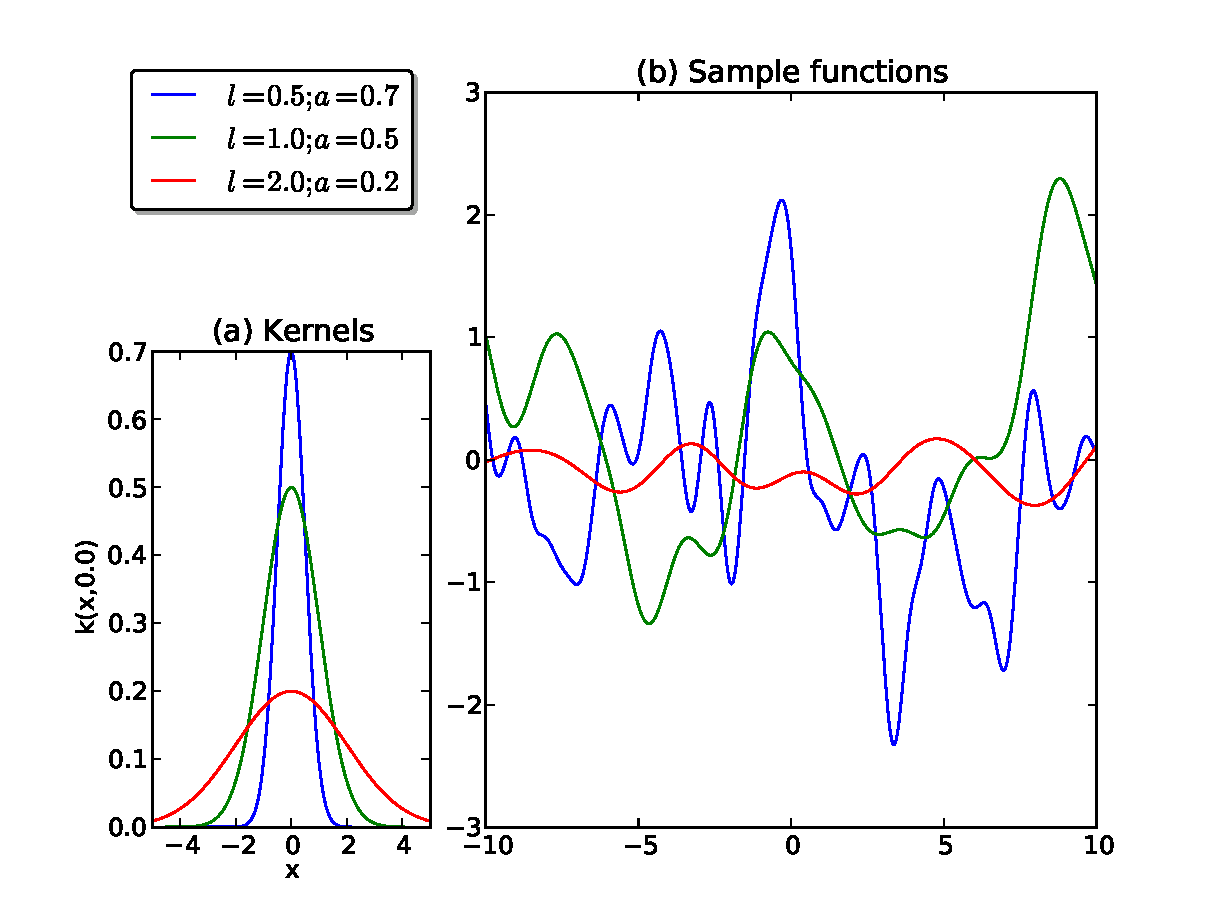
\includegraphics[width=10cm,keepaspectratio]{diagrams/SE_cov.pdf}
		%\includegraphics[width=0.7\textwidth,keepaspectratio]{diagrams/PCA2.eps}
		\includegraphics[width=0.7\textwidth,keepaspectratio]{PCA2.eps}
		\rule{35em}{0.5pt}
	\caption[Principal component analysis of time series data ]
		{Principal component analysis of gene expression time series data}
	\label{fig:PCA_time_series}
\end{figure}

\subsection{Transcription Factors}
From different data sources we found different number/list of transcription factor. \cite{Inmaculada:2007} 
build a database named \textit{C. elegans} differential gene expression database 
(EDGEdb) which contains the sequence information about 934 predicted transcription factors and
their DNA binding domains. Initially we took these 934 transcription factors for our baseline experimental setup
but we also kept the opening to deal with any number of transcription factor depending on the requirement/ 
update of the sequence information of transcription factors.

\subsection{Connectivity Information}
\cite{WormNet} is a gene network of protein-encoding genes for \textit{C. elegans} based on based on probabilistic function
and modified Bayesian integration. They have considered 15,139 genes and 999,367 linkages between genes 
associated with a log-likelihood score (LLS). These measured scores represents a true functional linkage between a pair 
of genes \cite{Lee:2007}.
The linkage between two genes were measured based on the following evidence codes(\cite{WormNet})-
\begin{itemize}
 \item CE-CC: 	Co-citation of worm gene
 \item CE-CX: 	Co-expression among worm genes
 \item CE-GN: 	Gene neighbourhoods of bacterial and archaeal orthologs of worm genes
 \item CE-GT: 	Worm genetic interactions
 \item CE-LC: 	Literature curated worm protein physical interactions
 \item CE-PG: 	Co-inheritance of bacterial and archaeal orthologs of worm genes
 \item CE-YH: 	High-throughput yeast 2-hybrid assays among worm genes
 \item DM-PI: 	Fly protein physical interactions
 \item HS-CC: 	Co-citation of human genes
 \item HS-CX: 	Co-expression among human genes
 \item HS-DC: 	Co-occurrence of domains among human proteins
 \item HS-LC: 	Literature curated human protein physical interactions
 \item HS-MS: 	human protein complexes from affinity purification/mass spectrometry
 \item HS-YH: 	High-throughput yeast 2-hybrid assays among human genes
 \item SC-CC: 	Co-citation of yeast genes
 \item SC-CX: 	Co-expression among yeast genes
 \item SC-DC: 	Co-occurrence of domains among yeast proteins
 \item SC-GT: 	Yeast genetic interactions
 \item SC-LC: 	Literature curated yeast protein physical interactions
 \item SC-MS: 	Yeast protein complexes from affinity purification/mass spectrometry
 \item SC-TS: 	Yeast protein interactions inferred from tertiary structures of complexes
\end{itemize}

We have constructed the connectivity matrix between genes and associated transcription factors 
from the gene to gene linkage and log-likelihood scores. 
We choose Co-expression among worm genes (CE-CX),
High-throughput yeast 2-hybrid assays among worm genes (CE-YH),
Literature curated human protein physical interactions (HS-LC) and 
High-throughput yeast 2-hybrid assays among human genes (HS-YH) to start our experiments.
But if needed we can consider any of the evidence to reconstruct the connectivity matrix.
From the gene list we have picked the protein-coding genes (i.e. transcription factors) and later 
binarized it. If there is an associated LLS value between a gene and a transcription factor we set the value '1' and 
'0' otherwise.

\section{Result Analysis}
We have developed a $R$ based tool $chipDyno$ for the identification of 
quantitative prediction of regulatory activities of the gene specific TFA through posterior estimation.
The $chipDyno User Guide$ attached at the end of this report explains different functionality 
of this tool and working pathway.

For \textit{C. elegans} gene specific TFA is quite a new experiments. So we didn't find any other result to
consider a baseline and compare our result. 

\begin{figure}
%\begin{figure}[htbp]
	\centering
		%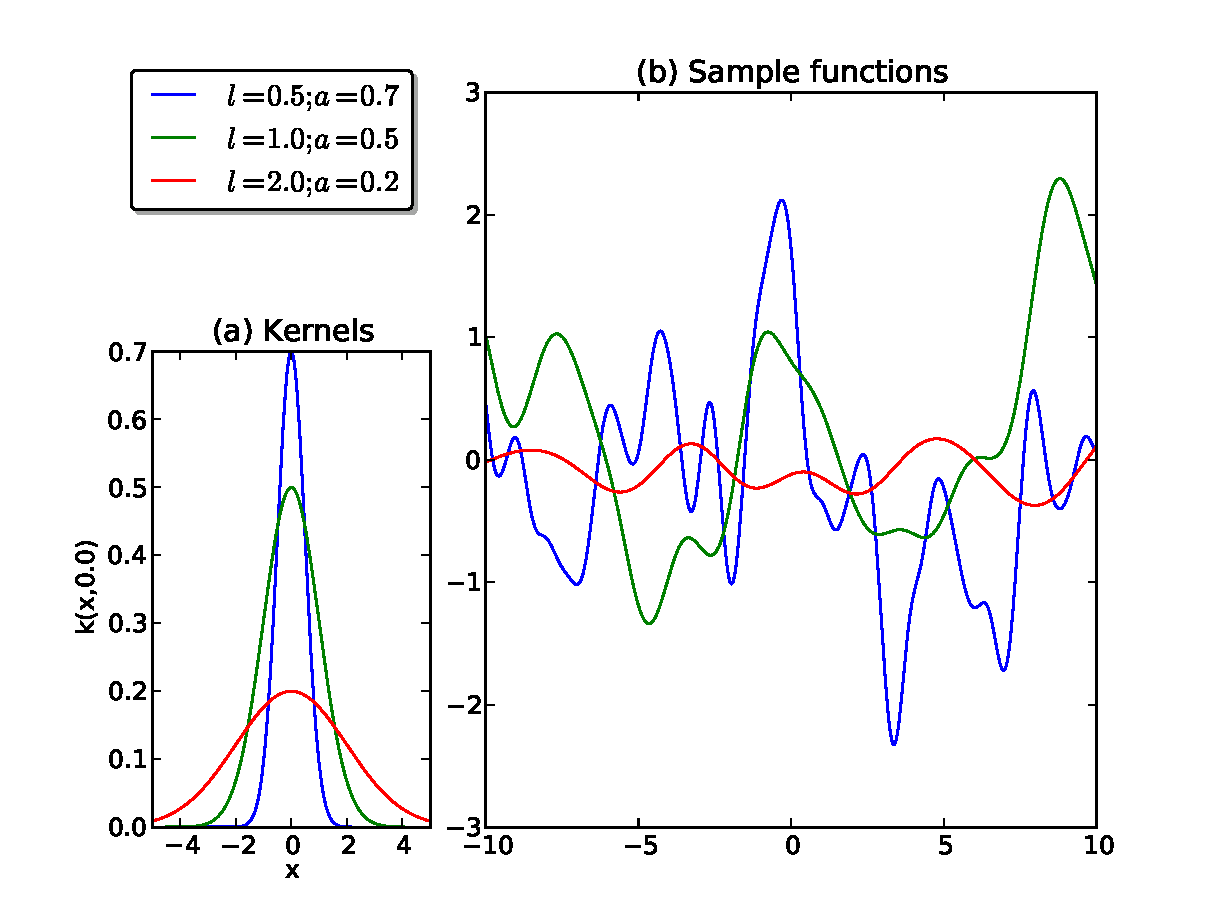
\includegraphics[width=10cm,keepaspectratio]{diagrams/SE_cov.pdf}
		%\includegraphics[width=\textwidth,keepaspectratio]{diagrams/ZK370_2_3.eps}
		\includegraphics[width=\textwidth,keepaspectratio]{ZK370_2_3.eps}
		\rule{35em}{0.5pt}
	\caption[Gene Specific transcription factor activity of ZK370.2]
		{Gene Specific transcription factor activity of ZK370.2}
	\label{fig:TFA_of_of_ZK370.2}
\end{figure}

According to \cite{WormNet} the number of gene of \textit{C. elegans} is 15,139 
and \cite{Inmaculada:2007} presented 934 transcription factors. All the network motif, i.e.
autoregulation, multi-component loop, feedforward loop, single input, multi-input motif, regulator chain
were visible for transcription factor activity. So it was a mammoth task to choose all the transcription
factors and show their activity. Rather we choose some random transcription factor and tried to 
find out its activity on different genes.

\begin{figure}
%\begin{figure}[htbp]
	\centering
		%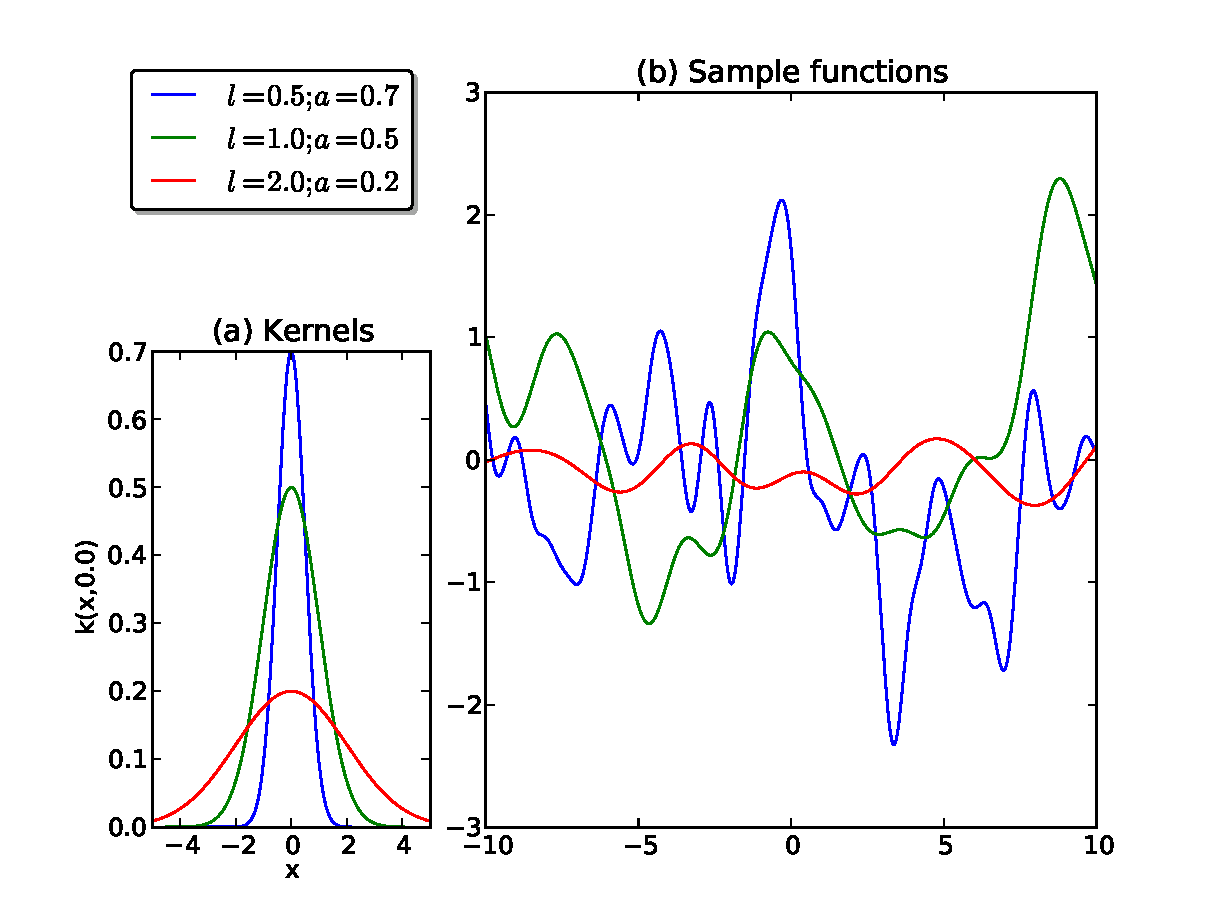
\includegraphics[width=10cm,keepaspectratio]{diagrams/SE_cov.pdf}
		%\includegraphics[width=\textwidth,keepaspectratio]{diagrams/T20B12_8_3.eps}
		\includegraphics[width=\textwidth,keepaspectratio]{T20B12_8_3.eps}
		\rule{35em}{0.5pt}
	\caption[Gene Specific transcription factor activity of T20B12.8.3]
		{Gene Specific transcription factor activity of T20B12.8.3}
	\label{fig:TFA_of_of_T20B12_8_3}
\end{figure}

As a random sample we choose transcription factor ZK370.2 and tried to find its activity on different
genes. Figure \ref{fig:TFA_of_of_ZK370.2} shows that ZK370.2 can act on C37C3.2, Y105E8B.3, Y45F10B.3,
C34F11.3, F26E4.6 and T24G10.2. In the dataset we had three replication of same experimental setup and 
it outcome. We also tried to run our experiments three times and collect the result individually. 
Later we plot all the outcome together.
From the outcome of our experimental result we can say that for some cases (i.e. F26E4.6 and T24G10.2)
the result is very flat and doesn't looks so informative but some of the results represents TFAs varies 
notably over time (i.e. C37C3.2 and Y45F10B.3). 
Perhaps these are the genes which regulates significantly by this transcription
factor. For some cases the error bar is quite high. False positive could be an issue here. The magnitude 
of TFA also differs from one to another.
We picked another random transcription factor T20B12.8.3. Figure \ref{fig:TFA_of_of_T20B12_8_3} shows its
activity on different genes.

\subsection{Gene with multiple regulators}
For the case of multi input motif a single gene could be regulated by multiple transcription factor. Our 
developed tool can determine the posteriori of the relative weight for the different transcription
factors regulating the genes. Table \ref{table:Genes_regulated_by_multiple_TF} shows some examples.
Gene C44B12.5 can be regulated by transcription factor Y116A8C.35 and F33A8.3. While gene
Y105E8B.3 is regulated by T20B12.8, F33A8.3, Y116A8C.35, F11A10.2 and C16A3.7. Though for some cases 
the expression level is quite low and noise margin is significantly high but we can rank these 
gene using \cite{Kalaitzis:2011}.


\begin{table}
	\centering
\begin{tabular}{l l }
      \toprule
      \textbf{Gene Name} & \textbf{Regulators activity} \\
      \midrule
	      {\color{green}C44B12.5} & {\color{blue} Y116A8C.35 }= $ 1.719797 \pm 3.493205 $, \\ 
				    & {\color{blue}F33A8.3} = $ 1.415785 \pm 3.492985$ \\~\\

		{\color{green}Y105E8B.3} & {\color{blue} Y54G2A.1} = $ 0.07157665 \pm 1.2222137 $ \\
		  & {\color{blue} F33D11.12} = $ 0.03861905 \pm 0.7252534 $ \\
 		  & {\color{blue} ZK370.2} = $ -1.20157055 \pm  2.0318513 $\\~\\
		    
	      {\color{green} Y105E8B.3} & {\color{blue} T20B12.8 } = $ 0.25474933 \pm  2.5665869 $ \\
		  			& {\color{blue} F33A8.3 } = $ 0.11619828  \pm  3.5107742 $ \\
 		  			& {\color{blue} Y116A8C.35 } = $ 0.03289664 \pm  3.8071374 $ \\
					& {\color{blue} F11A10.2 } = $ 0.03016348 \pm 1.7737585 $ \\
 		  			& {\color{blue} C16A3.7  } = $ 0.01883489 \pm  $ 0.9431105\\

  \bottomrule
  \end{tabular}
	  \caption[Genes regulated by multiple TF]
		  {Genes regulated by multiple TF}
	  \label{table:Genes_regulated_by_multiple_TF}
\end{table}

\subsection{Different clusters and related active TF}
\cite{Cossins:2007} was also trying to some clusters analysis of the genes based on different
phenotype and its subsequent activities of the cell properties\footnote{The result wasn't published but we came to know 
about it through some discussions.}.
Here are the basic clusters and some of the phenotype properties:

\begin{figure}
	\centering
		%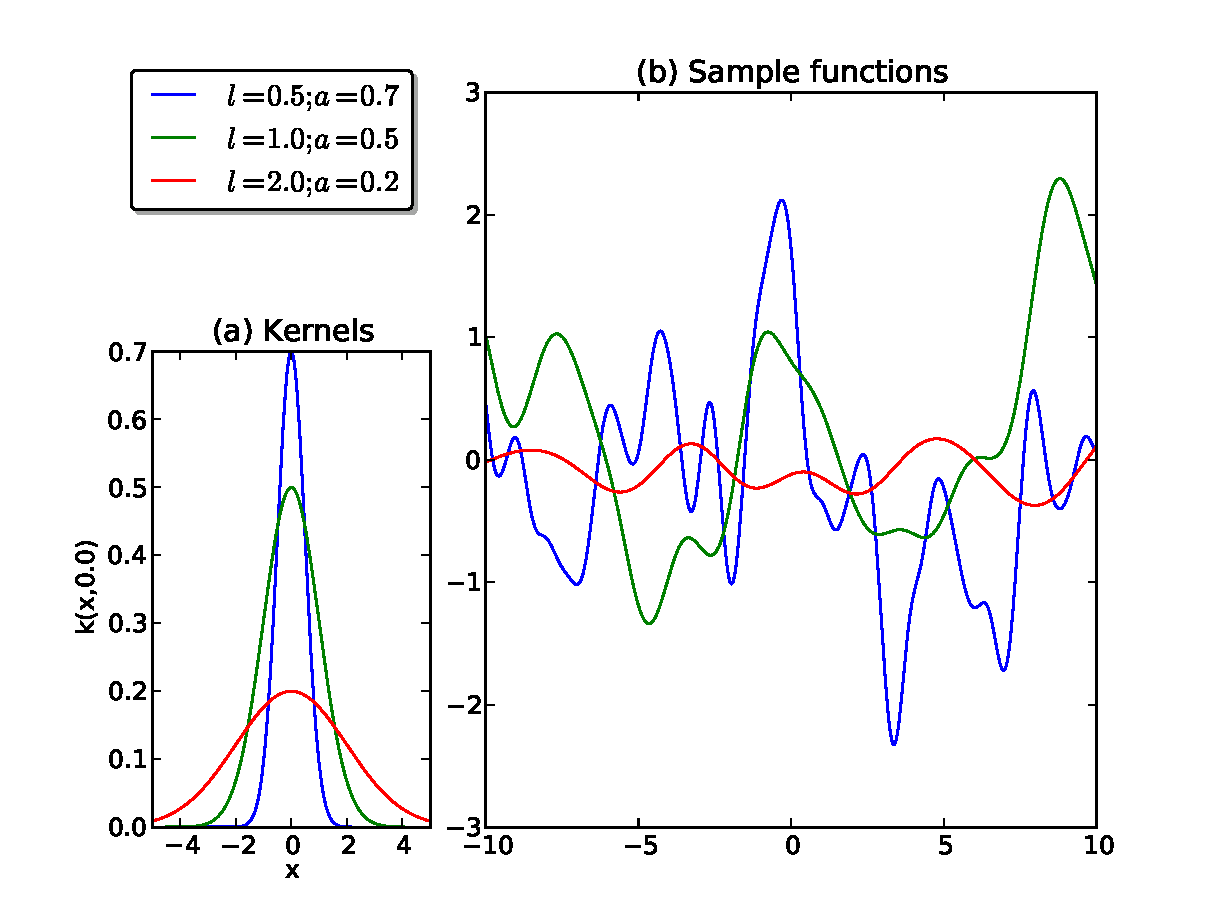
\includegraphics[width=10cm,keepaspectratio]{diagrams/SE_cov.pdf}
		%\includegraphics[width=\textwidth,keepaspectratio]{diagrams/T20B12_8_3.eps}
		%\includegraphics[scale=.5]{diagrams/mcd3.eps}
		\includegraphics[scale=.5]{mcd3.eps}
		\rule{35em}{0.5pt}
	\caption[Clustering of TF]
		{Clustering of TF}
	\label{fig:Clustering_TF}
\end{figure}

\textbf{Cluster 1 - Chill upregulated} basically related with
cell morphogenesis, cell growth, regulation of cell size, electron transport
regulation of cell growth, generation of precursor metabolites and energy,
anatomical structure morphogenesis, cellular metabolic process, proteolysis,
etc.

\textbf{Cluster 2 - Chill late upregulated} related with
chromosome organization and biogenesis, DNA packaging, chromatin architecture
chromatin modification, negative regulation of developmental process, 
chromatin remodelling, regulation of developmental process, DNA metabolic process
larval development (sensu Nematoda), organelle organization and biogenesis, 
post-embryonic development etc.

\textbf{Cluster 3 - Chill downregulated genes} related with
amino acid and derivative metabolic process, carboxylic acid metabolic process,
organic acid metabolic process, fatty acid metabolic process,
amino acid metabolic process, monocarboxylic acid metabolic process, etc. 
Rest of the genes were placed in the group 'Others'.

Figure \ref{fig:Clustering_TF} shows heat map generated from DNA 
microarray data to reflect the gene expression values at
different temperature and their basic clusters \cite{Cossins:2007}\footnote{Some portion of the result
is unpublished result; came to know through a presentation}.
Based on the above clusters we have tried to find out the the transcription factors
active for different clusters. We have managed to find out the active
transcription factor for each clusters and Table \ref{table:Active_TF_diff_clusters}
shows the numbers.


\begin{table}
  \centering
  \begin{tabular}{l l }
    \toprule
    \textbf{Clusters} & \textbf{Active TF} \\
    \midrule
    1. {\color{blue}Chill upregulated} & {\color{green}\bf 6} \\ 
    2. {\color{blue}Chill late upregulated} & {\color{green}\bf245} \\ 
    3. {\color{blue}Chill downregulated} & {\color{green}\bf128} \\
    4. {\color{blue} Others} & {\color{green}\bf 203} \\
  \bottomrule
  \end{tabular}
  \caption[Active TF on different clusters]
	  {Active TF on different clusters}
  \label{table:Active_TF_diff_clusters}
\end{table}


\section{Ranking Differentially expressed gene expressions}
\cite{Kalaitzis:2011} analysed the time series gene expression and filter the quiet or inactive genes
from the differentially expressed genes. They have developed the model considering the temporal nature of data 
using Gaussian process. We have used this model to rank our time series gene expression and ranked the 
differentially expressed gene expressions. 
We tried to rank the three replicates of our data separately and later determine the
Pearson correlation between ranking score of different samples.

\begin{figure}
	\centering
		%\includegraphics[scale=.7,keepaspectratio]{diagrams/RankingScoreLogValue.eps}
		\includegraphics[scale=.7,keepaspectratio]{RankingScoreLogValue.eps}
		\rule{35em}{0.5pt}
	\caption[Pearson's correlation between different ranking scores]
		{Pearson's correlation between different ranking scores}
	\label{fig:ranking_scores}
\end{figure}

Figure \ref{fig:ranking_scores} shows the Pearson correlation between different ranking scores.
The correlation coefficient for all three relations (between sample 1 and sample 2, sample 2 and sample 3 and
sample 3 and sample 1) were quite high. Which indicates the similarity of 
differentially expressed genes and quiet genes of different samples or replication of time series data.
So, if required, based on these ranking we can easily filter out some of the quiet genes and keep the
other genes for further experiments.


%\section{Convetional Approach of Clustering and related TFs}